% !TEX root = ../../mat_738_alggeo.tex
\newpage
\section{Varieties}
\subsection{Introduction}

One could define Algebraic Geometry as the study of solutions to systems of polynomial equations. The early history of Algebraic Geometry was focused on what we will eventually know as affine varieties, especially the simplest cases plane algebraic curves, e.g. lines, circles, parabolas, ellipses, hyperbolas, and cubic curves. The development of Algebraic Geometry was slow, due to cumbersome language, notation, varying approaches, and especially varying or ineffective definitions. However motived by work in various fields including Complex Analysis, (Algebraic) Topology, Number Theory, and especially Commutative Algebra, Algebraic Geometry developed rapidly. Modern Algebraic Geometry is due largely to the development of the theory of sheaves and schemes by Grothendieck and Serre, but is also due to the contribution of many others such as  Zariski, \v{C}ech, Leray, Cartan, et al.. 



% Affine Varieties
\subsection{Affine Varieties}

Let $k$ be a fixed algebraically closed field.\footnote{Note that much of elementary Algebraic Geometry, the requirement that $k$ be algebraically closed is unnecessary, and $k$ being an arbitrary field, or even simply an integral domain would suffice.} Often, we will focus on the case where $k= \C$.


\begin{dfn}[Affine $n$-space]
Denote by $k^n$ the set of ordered $n$-tuples of elements of $k$. Then define $\A_k^n:= k^n$, called affine $n$-space over $k$. Note that this is also denoted $\A^n(k)$ or simply $\A^n$ when $k$ is understood. 
\end{dfn}


For ease of notation, we often denote the polynomial ring $k[x_1,\ldots,x_n]$ simply by `$A$'. We can think of elements of $A:= k[x_1,\ldots,x_n]$ as being functions $f: \A^n \to k$ via $(k_1,\ldots,k_n) \mapsto f(k_1,\ldots,k_n)$, i.e. via evaluation; that is, given $f \in A$ and $P=(k_1,\ldots,k_n)$, we have $f(P)= f(k_1,\ldots,f_n) \in k$. This allows us to consider the vanishing set of the polynomial $f$. 


\begin{dfn}[Zero Set]
For $f \in A:= k[x_1,\ldots,x_n]$, define $Z(f):= \{ P \in \A^n \;|\; f(P)=0 \}$, called the zero set of $f$. For $T \subseteq A$, we define the zeros of $T$, denoted $Z(T)$, by 
	\[
	Z(T):= \bigcap_{f \in T} Z(f)= \{ P \in \A^n \;|\; f(P)=0 \text{ for all } f \in T \}.
	\]
If $T= \{f_1,\ldots,f_r\}$, we will often write $Z(T)= Z(f_1,\ldots,f_r)$. 
\end{dfn}


Note the underlying field $k$ does matter here. For example, $Z(x^2+1)= \emptyset$ if $k= \R$ but if $k= \C$, then $Z(x^2+1)= \{ \pm i \}$. As another example in $\R^2$, $Z(y-x^2, x-y^2)$ consists of two points, namely the points $(0,0), (1,1)$ of intersection, see Figure~\ref{fig:algsetex}. However if $k= \C^2$, then $Z(y-x^2,x-y^2)$ consists of four points: $(0,0), (1,1), (-\zeta_3,\zeta_3^2), (\zeta_3^2,-\zeta_3)$, where $\zeta_3$ is a primitive cube root of unity. 

	\begin{figure}[h!]
	\centering
	\begin{tikzpicture}[scale=1.1]
	%\clip (-3,-3) rectangle (5cm,5cm);
	\coordinate (Origin)   at (0,0);
    	\coordinate (XAxisMin) at (-3,0);
    	\coordinate (XAxisMax) at (3,0);
    	\coordinate (YAxisMin) at (0,-3);
    	\coordinate (YAxisMax) at (0,3);
    	
	\draw [thin,-latex] (XAxisMin) -- (XAxisMax) node[right] {\footnotesize$x$};
    	\draw [thin,-latex] (YAxisMin) -- (YAxisMax) node[above] {\footnotesize$y$};
	
	\draw[scale=0.5,domain= -2.5:2.5,smooth,variable=\x,blue,thick] node at (3.5,4.5) {$y^2=x^3$} plot ({\x},{\x*\x});
	\draw[scale=0.5,domain= -2.5:2.5,smooth,variable=\x,red,thick] node at (2.5,-2.5) {$x=y^2$} plot ({\x*\x},{\x});
	\end{tikzpicture}
	\caption{If $k= \R^2$, then the set $Z(y-x^2, x-y^2)$ is the intersection of $y= x^2$ with $x= y^2$. \label{fig:algsetex}}
	\end{figure}


We now have enough to define the basic building block of Algebraic Geometry.


\begin{dfn}[Algebraic Set]
A subset $Y \subseteq \A^n$ is called an algebraic set if and only if there exists a subset $T \subseteq A$ such that $Y= Z(T)$. We also refer to such sets as affine (algebraic) varieties. 
\end{dfn}


That is, a set of points $Y$ is an algebraic set if $Y$ is a set of common zeros for a collection of polynomials $T$. 


\begin{ex} \label{ex:emptyandwhole} \hfill
\begin{enumerate}[(i)]
\item  The emptyset, $\emptyset$, is algebraic since $\emptyset= Z(1)$, where $f= 1$ is the constant polynomial $f= 1$. Furthermore, $\A^n$ is an algebraic set since $\A^n= Z(0)$, where $f= 0$ is the zero polynomial. 

\item Any single point $P=(k_1,\ldots,k_n) \in \A^n$ is an algebraic set since $\{P\}= Z(x_1-k_1,\ldots,x_n-k_n)$. In fact, any \emph{finite} collection of points is algebraic, c.f. Proposition~\ref{prop:basic_affine}. [One should check that you can write down an explicit polynomial to confirm this.] 

\item The set $\{ (x,y) \colon y-f(x)= 0 \}$, where $f(x)$ is a polynomial, is trivially algebraic. But this is precisely the graph of the function $y= f(x)$. For example, the cubic $y= x^3$ is algebraic (meaning its graph). This easily generalizes to $y= f(x_1,\ldots,x_n)$, where $f(x_1,\ldots,x_n)$ is a polynomial. Furthermore considering the graph of $Ax^2+By^2+Cz^2+Dxy+Exz+Fyz+Gx+Hy+Iz+J=0$, we see that the graph of every quadratic surface an algebraic surface, e.g. the cone, ellipsoid, cylinder, hyperboloid, etc.. 
	\begin{figure}[h!]
	\centering
	\begin{tikzpicture}[scale=0.9]
	\coordinate (Origin)   at (0,0);
    	\coordinate (XAxisMin) at (-3,0);
    	\coordinate (XAxisMax) at (3,0);
    	\coordinate (YAxisMin) at (0,-3);
    	\coordinate (YAxisMax) at (0,3);	
	
	\draw [thin,-latex] (XAxisMin) -- (XAxisMax) node[right] {\footnotesize$x$};
    	\draw [thin,-latex] (YAxisMin) -- (YAxisMax) node[above] {\footnotesize$y$};

	\draw[scale=0.5,domain= -1.8:1.8,smooth,variable=\x,blue,thick] node at (3.3,4.5) {$y=x^3$} plot ({\x},{\x^3});		
	\end{tikzpicture} \hfill
	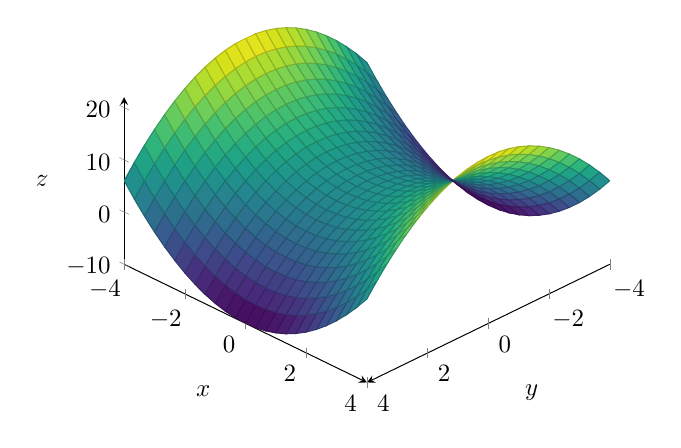
\begin{tikzpicture}[scale=0.9]
    	\begin{axis}[
	colormap name={viridis},
	axis lines= left,
	xtick={-4,-2,...,4}, % \empty
	ytick={-4,-2,...,4},
	ztick={-20,-10,...,20},
	xlabel=$x$,
	ylabel=$y$,
	zlabel=$\mathbin{\rotatebox[origin=c]{90}{$z$}}$,
   	smooth, % samples = 50,
  	domain=-4:4,
	view={-45}{-45}
  	]
  	\addplot3[surf] {x^2-y^2+6};
 	\end{axis}	
	\end{tikzpicture}
	\caption{One the left, the algebraic set given by the curve $y=x^3$ (not including axes). On the right, the algebraic set given by $z=x^2-y^2+6$ (not including axes).}
	\end{figure}

\item A `line glued to a circle' is an algebraic set, i.e. the image in Figure~\ref{fig:linegluecirc} (excluding the axes) is an algebraic set since it represents the set $Z((x^2+y^2-1)(y-2))=\{ (x,y) \colon (x^2+y^2-1)(y-2) \}$. Why? If $(x^2+y^2-1)(y-2)=0$, then either $x^2+y^2=1$, in which case the point lies on the circle, or $y-2=0$ in which case the point $(x,y)$ lies on the line $y=2$. In fact, even the coordinate axes are algebraic sets because together they are $Z(xy)$, by a similar reasoning. 
	\begin{figure}[h!]
	\centering
	\begin{tikzpicture}
	\coordinate (Origin)   at (0,0);
    	\coordinate (XAxisMin) at (-3,0);
    	\coordinate (XAxisMax) at (3,0);
    	\coordinate (YAxisMin) at (0,-3);
    	\coordinate (YAxisMax) at (0,3);	
	
	\draw [thin,-latex] (XAxisMin) -- (XAxisMax) node[right] {\footnotesize$x$};
    	\draw [thin,-latex] (YAxisMin) -- (YAxisMax) node[above] {\footnotesize$y$};

	\draw[domain= -1.5:1.5,samples=50,variable=\x,blue,thick] node at (1.2,1.2) {} plot ({\x},{sqrt((1.5)^2-(\x)^2)});
	\draw[domain= -1.5:1.5,samples=50,variable=\x,blue,thick] node at (1.2,1.2) {} plot ({\x},{-sqrt((1.5)^2-(\x)^2)});		
	\draw[domain= -2.5:2.5,smooth,variable=\x,blue,thick] node at (1.2,1.2) {} plot ({\x},{1.5});	
	\end{tikzpicture}
	\caption{The algebraic set given by a `line glued to a circle.' \label{fig:linegluecirc}}
	\end{figure}


\item The set of all $n \times n$ matrices can be identified with the set $\C^{n^2}$. This space contains many subsets of interest. For example, the matrices of determinant 1, SL$_n(\C)$, forms an affine algebraic variety in $\C^{n^2}$ because it is the vanishing set of the polynomial given by $\Delta - 1$, where
	\[
	\Delta(x_{ij})= \det 
	\begin{pmatrix} 
	x_{11} &  \cdots & x_{1n} \\ 
	\vdots & \ddots & \vdots \\
	x_{n1} & \cdots & x_{nn}
	\end{pmatrix}
	\]
is the determinant. In fact, a determinantal variety is the set of all matrices (considered as a subset of $\C^{n^2}$) of rank at most $k$. For $k \geq n$, the determinantal variety is the whole space $\C^{n^2}$. But for $k<n$, the rank of a matrix $A$ is at most $k$ if and only if all its $(k+1) \times (k+1)$ subdeterminants vanish. But as these subdeterminants are polynomials in the variables $x_{ij}$, the set of matrices of rank at most $k$ is an affine algebraic variety.  \xqed
\end{enumerate}
\end{ex}


Of course, not all sets are algebraic. Not even all curves in $\R^2$ are algebraic, as the following exercise demonstrates. 


\begin{exc} \hfill
\begin{enumerate}[(a)]
\item Prove that in $\A^2_\R$, the graph of $y= \sin x$ is not an algebraic set, i.e. prove the set $\{ (x,y) \colon y= \sin x \}$ is not algebraic. [{\em Hint: The graph intersects the $x$-axis at infinitely many points, but single variable polynomials have finitely many roots.}]

\item Prove that in $\A^2_\R$, the graph of $y= e^x$ is not an algebraic set, i.e. prove the set $\{ (x,y) \colon y= e^x \}$ is not an algebraic set. [{\em Hint: $e^x$ grows `faster' than any polynomial, i.e. $\displaystyle \lim_{x \to \infty} \dfrac{e^x}{x}= \infty$.}]

\item Prove that the open ball in the usual Euclidean topology on $\C^n$ is not an algebraic set by showing that every affine algebraic variety in $\C^n$ is closed in the Euclidean topology. [{\em Hint: Polynomials are continuous functions from $\C^n$ to $\C$, so their zero sets are closed.}] Explain then why the set of invertible matrices, GL$_n(\C)$ is not an affine algebraic variety.
\end{enumerate}
\end{exc}


Note that if $N \subseteq M$, then $Z(M) \subseteq Z(N)$, since any polynomial which  vanishes on all of $M$ certainly vanishes on all of $N$. Combining this with the Hilbert Basis Theorem: if $R$ is noetherian, then $R[x_1,\ldots,x_n]$ is noetherian, we obtain the following result.


\begin{prop} \label{prop:basic_affine} \hfill
\begin{enumerate}[(a)]
\item Let $T \subseteq A$ and $J$ be the ideal generated by $T$, then $Z(T)= Z(J)$. In particular, every algebraic set in $\A^n$ is of the form $Z(J)$ for some ideal $J$ of $A$. 
\item Every algebraic set in $\A^n$ is of the form $Z(T)$ for some finite set $T \subseteq A$.
\end{enumerate}
\end{prop}

\pf \hfill
\begin{enumerate}[(a)]
\item Since $T$ generates $J$, we know that $T \subseteq J$ which immediately implies $Z(J) \subseteq Z(T)$. For the reverse inclusion, let $P \in Z(T)$ so that for all $f \in T$, $f(P)=0$. If $g \in J$, we have $g= \sum_{i=1}^m a_i f_i$, where $a_i \in A$, $f_i \in T$. But then we have
	\[
	g(P)= \sum_{i=1}^m a_i(P) f_i(P)= \sum_{i=1}^m a_i(P) \cdot 0= 0.
	\]
Therefore, $Z(T)= Z(J)$. By definition, $Y \subseteq \A^n$ is algebraic if and only if there is $T \subseteq A$ with $Y= Z(T)$. Taking $J:= \langle T \rangle$, the second claim follows. 


\item Since $k$ is a field, we know that $A= k[x_1,\ldots,x_n]$ is noetherian by the Hilbert Basis Theorem. Recall that every ideal in a noetherian ring is finitely generated (in fact this is equivalent to the definition).  By (a), we know that $Y \subseteq \A^n$ is algebraic if and only if $Y= Z(J)$ for some ideal $J$ of $A$. But as $A$ is noetherian, we can find a finite number of generators, say $T:=\{f_1,\ldots, f_r\}$, for $J$. Therefore, $Y= Z(J)=Z(\langle T \rangle)=Z(T)= Z(f_1,\ldots,f_r)$, as desired. \qed \\
\end{enumerate}


Our goal is to build an underlying topological structure with which to work. This will form the basis for much of what is to come later. But first, we will need a proposition. 


\begin{prop} \label{prop:closedset} \hfill
\begin{enumerate}[(a)]
\item The empty set and whole space are algebraic sets. 
\item The finite union of algebraic sets is algebraic.
\item The intersection of any algebraic sets is algebraic. 
\end{enumerate}
\end{prop}

\pf \hfill
\begin{enumerate}[(a)]
\item Recall from Example~\ref{ex:emptyandwhole} that $\emptyset= Z(1)$ and $\A^n= Z(0)$ are algebraic sets. 

\item By induction, it suffices to prove that the union of two algebraic sets is algebraic. Suppose that $S_1,S_2$ are algebraic sets. Then by Proposition~\ref{prop:basic_affine}, we know that $S_1= Z(T_1)$ and $S_2= Z(T_2)$ for some $T_1,T_2 \subseteq A$. We need show that $S_1 \cup S_2= Z(T_1) \cup Z(T_2)= Z(T)$ for some set $T$. We shall show that $Z(T_1) \cup Z(T_2)= Z(T_1T_2)$, i.e. $T= T_1T_2= \{ t_1t_2 \colon t_1 \in T_1, t_2 \in T_2 \}$ works, so that again by Proposition~\ref{prop:basic_affine}, $S_1 \cup S_2$ is algebraic. 

To see that $Z(T_1) \cup Z(T_2) \subseteq Z(T_1T_2)$, let $P \in Z(T_1) \cup  Z(T_2)$. But then $P \in Z(T_1)$ or $Z(T_2)$. Without loss of generality, suppose $P \in Z(T_1)$. Any element of $T_1T_2$ is of form $fg$, where $f \in T_1, g \in T_2$. But then $P \in Z(T_1T_2)$. 

To see that $Z(T_1T_2) \subseteq Z(T_1) \cup Z(T_2)$, choose $P \in Z(T_1T_2)$. We will show that if $P \notin Z(T_1)$ then $P \in Z(T_2)$. So suppose $P \notin Z(T_1)$. Then there is $f \in T_1$ with $f(P) \neq 0$. Choose any $g \in T_2$. Now $fg \in T_1T_2$ so $(fg)(P)= 0$. But $0= (fg)(P)= f(P)g(P)$. We know $f(P) \neq 0$ whenever$k$ is an integral domain, so that we must have $g(P)= 0$. As $g \in T_2$ was arbitrary, then $P \in Z(T_2)$.
 
\item Suppose $\{S_i\}_{i \in \mathcal{I}}$ is a collection of algebraic sets. Then for each $i \in \mathcal{I}$, we know that $S_i= Z(T_i)$ for some $T_i \subseteq A$. But then we have
	\[
	\bigcap_{i \in \mathcal{I}} S_i= \bigcap_{i \in \mathcal{I}} Z(T_i) = Z \left( \bigcup_{i \in \mathcal{I}} T_i \right),
	\]
where the last equality follows since $P \in Z(\bigcup_{i \in \mathcal{I}} T_i)$ if and only if every polynomial in every $T_i$ vanishes at $P$, i.e. $P \in \bigcap_{i \in \mathcal{I}} Z(T_i)$. \qed \\
\end{enumerate}


Notice that Proposition~\ref{prop:closedset} shows that the algebraic sets are precisely the closed sets in some topology, called the Zariski topology on $\A^n$.


\begin{dfn}[Zariski Topology]
The Zariski topology on $\A^n$ is defined by taking the open sets to be the complements of algebraic sets. 
\end{dfn}


\begin{ex}
What is the Zariski topology on $\A^1$? Since $k$ is a field, $A= k[x]$ is a PID, so every ideal in $A$ is principal. But by Propositon~\ref{prop:basic_affine}, every algebraic set $Y$ is of the form $Y= Z(J)$ for some ideal $J$. But then $Y=Z(f)$ for some polynomial. Since $k$ is algebraically closed, we can factor $f(x)$ as $f(x)= c(x-a_1)\cdots(x-a_n)$, where $c, a_1,\ldots,a_n \in k$. Therefore, $Z(f)= \{a_1,\ldots,a_n\}$. The closed sets in the Zariski topology are then $\emptyset$, $\A^1$, and all finite subsets. Therefore, the Zariski topology on $\A^1$ consists of $\emptyset$, $\A^1$, and the complements of finite subsets. But then every set which is not the whole set or $\emptyset$ contain all but finitely many elements of $k$. In particular, every two open sets intersect so that the Zarisiki topology on $\A^1$ is (extremely) not Hausdorff. \xqed
\end{ex}





















%\begin{ex}
% any point algebraic
% V(y-x^2,x-y^2) two points in \R^2 but 4 points in \C^2. Generally, B\'ezouts theorem number intersections curve degree m with degree n is mn in prokective space.
% twisted cubic: (t,t^2,t^3), V(y-x^2,z-x^3)
% Note all curves in \R^ are algebraic X= \{(x,y) \colon y- \sin x=0\}. SuppoSe X=V(S) for sume S subset R[x,y]. Then there is F \in S with F \neq 0 so X=V(S)= \cap f \in S V(f) \subseteq V(F). But the intersection of $X$ with horizontal line y-c=0 is infinteily for -1 \leq c \leq 1. Choose c with F(x,c) not zero polynomial and notice number of solutions is finite so not algebraic. 

%Method above works generally, if $C$ is algebaric affine plane curve and $L$ is line not contained in C, then L \cap C is iether empty or finite set of points 
%\end{ex}













